\documentclass[a4paper,12pt]{article}
\usepackage[a4paper,margin=1in,footskip=0.25in]{geometry}
\usepackage[utf8]{inputenc}

% science
\usepackage{amsmath}
\usepackage{array}
\usepackage{siunitx}

% layout
\usepackage{float}
\usepackage{parskip}
\usepackage{graphicx}
\usepackage{circuitikz}
\usepackage{longtable}
\usepackage{hyperref}
\usepackage{subfig}

\renewcommand{\arraystretch}{1.3}
\newcolumntype{P}[1]{>{\raggedright\arraybackslash}p{#1}}
\newcommand{\tptt}{$\times\,$}


\title{Empirically finding the value of absolute zero using the ideal gas law}
\author{Terry Qi}

\begin{document}

\maketitle

\section{Design}
\subsection{Introduction}
% When we were introduced to the unit Kelvin in chemistry, I was initially confused by the need of a

During a trip for the purpose of completing my duke of edinburgh, when we have reached the hilltop and was resting for the descent, my supervisor --- which happened to be a physics teacher, told us that because at higher attitude water boils easier, thus at a lower maximum temperature, hikers cannot rely on the boiling of the water to purify it. For I am a frequent hiker, I first pondered, then decided to dig into the reasoning of this phenomenon. Initially I thought to conduct the experiment of the effects of altitude against the boiling point of water, but weather conditions quickly brushed away that idea. Through my research it seems that it is the decrease in atmospheric pressure that causes decrease the temperature needed for boiling, therefore I decided to investigate the relationship between temperature and pressure, and accidentally realizing its connection to a fundamental quantity when I extrapolate the recession line. While I've been told in class that the temperature of absolute zero is not physically reachable and is only useful in calculations, I now have a simple yet powerful procedure that calculates this variable.


\subsection{Research Question}
\begin{quote}
    What is the relationship between the pressure of room air mixture against its temperature under constant volume and quantity?
\end{quote}

\subsection{Background}
% talk about gases and the ideal gas law
There exists a wide range of chemical reactions that includes a variety of gases as reactants or products. For the sake of stoichiometric analysis, it is heavily desirable to be able to measure the number of moles of a gas. To ease the calculations involved with millions of individual gas particle at the microscopic level, the field of kinetic theory of matter created a model of the ideal gas with optimistic attributes attached that still resembles real gases in the world.

The five assumptions of an ideal gas are that: (1) the gas molecule collisions are elastic, (2) the volume of the particles are negligible, (3) there exists no intermolecular forces between the particles, (4) the particles of a gas obey Newtonian motion and move with a range of speed and direction. These assumptions will be crucial in designing my experiment.

With the help of numerous scientists over the span of 200 years, the model of the ideal gas law can be summarized in figure \ref{fig:igl}.

\begin{figure}[H]
    \[
    PV = nRT
    \]
    \caption{The Ideal Gas Law}
    \label{fig:igl}
\end{figure}

The law contains the relationships between the four gaseous state quantities, each in their respective standard units: $P$ for Pressure, $V$ for Volume, $n$ for number of moles, and $T$ for temperature. We are interested in strictly the relationship between temperature and pressure, thus extracting from the law, we arrive to the relationship in figure \ref{fig:pt}, where $c$ is the proportionality constant. This relation is also initially discovered by Joseph Louis Gay-Lussac.

\begin{figure}[H]
    \[
    P = cT
    \]
    \caption{Pressure and Temperature relationship}
    \label{fig:pt}
\end{figure}

For there is a linear relationship between pressure and temperature, in the case of an ideal gas, I should measure a linear trend when graphing the gas pressure against its temperature, with an intercept of zero when the units are standard (Pascals and Kelvin).

% TODO: show graph
% https://www.jove.com/science-education/11147/ideal-gas-law

% its connection to the idea of absolute zero
However, by transposing the two axis (so that it is a Temperature against Pressure graph), extrapolating the linear relationship, where $k$ is a proportionality constant:
\[
    T = kP,
\]
can display an incredible result. The absolute zero is a theoretical measurement of temperature that sets the lower bound of the temperature scale. At the temperature, the movements of the gas particles are precisely zero, therefore the gas has zero outwards pressure. Therefore the y-intercept of the regression line (the temperature when pressure is zero), should be zero when using an standard unit such as Kelvin, and would measure the value of absolute zero in Celsius when the temperature unit is in Celsius.

% show graph

% TODO: flip graph


% potential implication
Additionally, the proportionality constant $k$ can be used to determine the boiling point of water at a range of attitudes. Suppose there exists a function $f$ that is a mapping between heights and the atmospheric pressure,


% how I would measure it
% potential source of errors


\subsection{Variables}
\paragraph{Independent Variable}
The temperature of the air mixture in unit Celsius

\paragraph{Dependent Variable}
The pressure of the air mixture in unit Pascal

\subsection{Control Variables}

% table here
\begin{longtable}{P{0.2\textwidth}|P{0.35\textwidth}|P{0.35\textwidth}}
Controls & Reason & How\\\hline
\end{longtable}

\subsection{Materials}

\begin{itemize}
    \item gas pressure measurement probe ($\pm 0.25\si{psi}$)
    \item 500ml glass beaker
    \item 2 $\times$ digital thermometer ($\pm 0.1\si{C}$)
    \item 2 $\times$ retort stands
    \item bunsen burner, tripod, and heating mat
    \item lighter
\end{itemize}

\subsection{Method}


\begin{enumerate}
    \item Setup the experiment as shown as in figure \ref{fig:exp}, using two retort stands \& clamps, the bunsen burner setup, and an empty 500ml glass beaker.
    \item Lift the two clamps holding the gas pressure measurement probe, 
    \item 

\end{enumerate}

\subsection{Diagrams}

\begin{figure}[H]
 \centering
 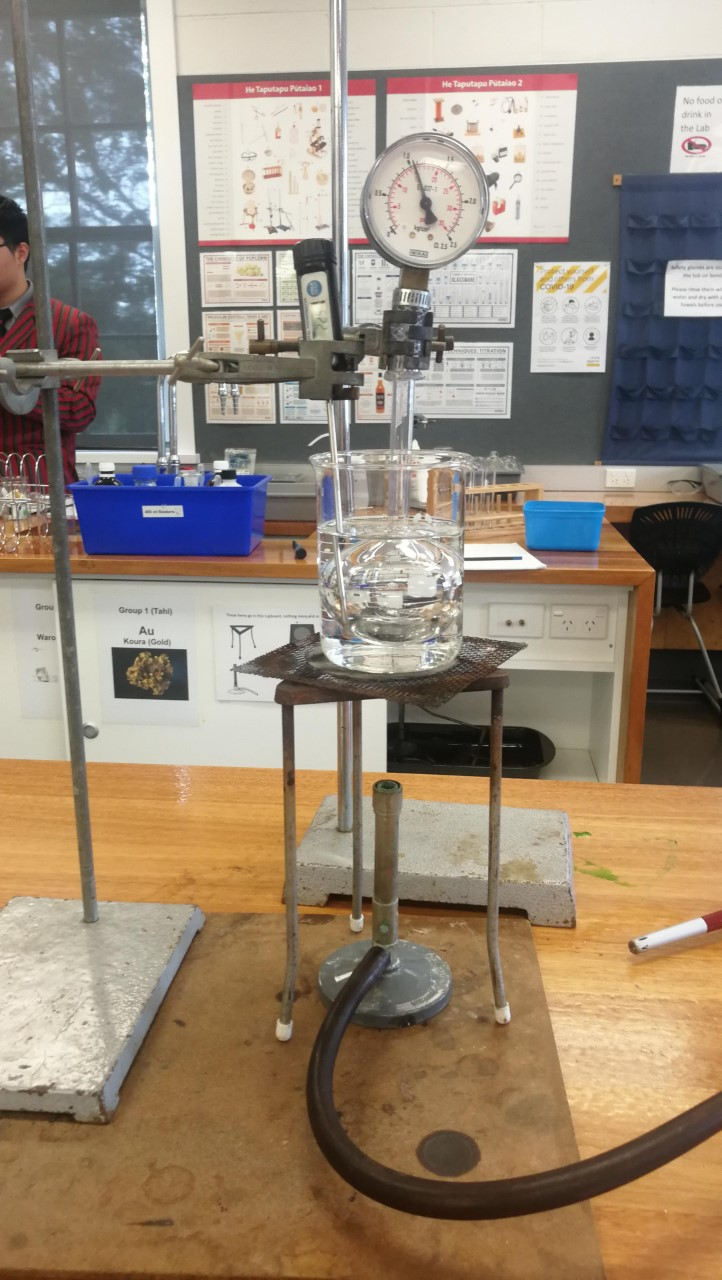
\includegraphics[scale=0.2]{assets/setup.jpg}
 \caption{The gas pressure measurement probe}
 \label{fig:gpmp}
\end{figure}

\begin{figure}[H]
 \centering
 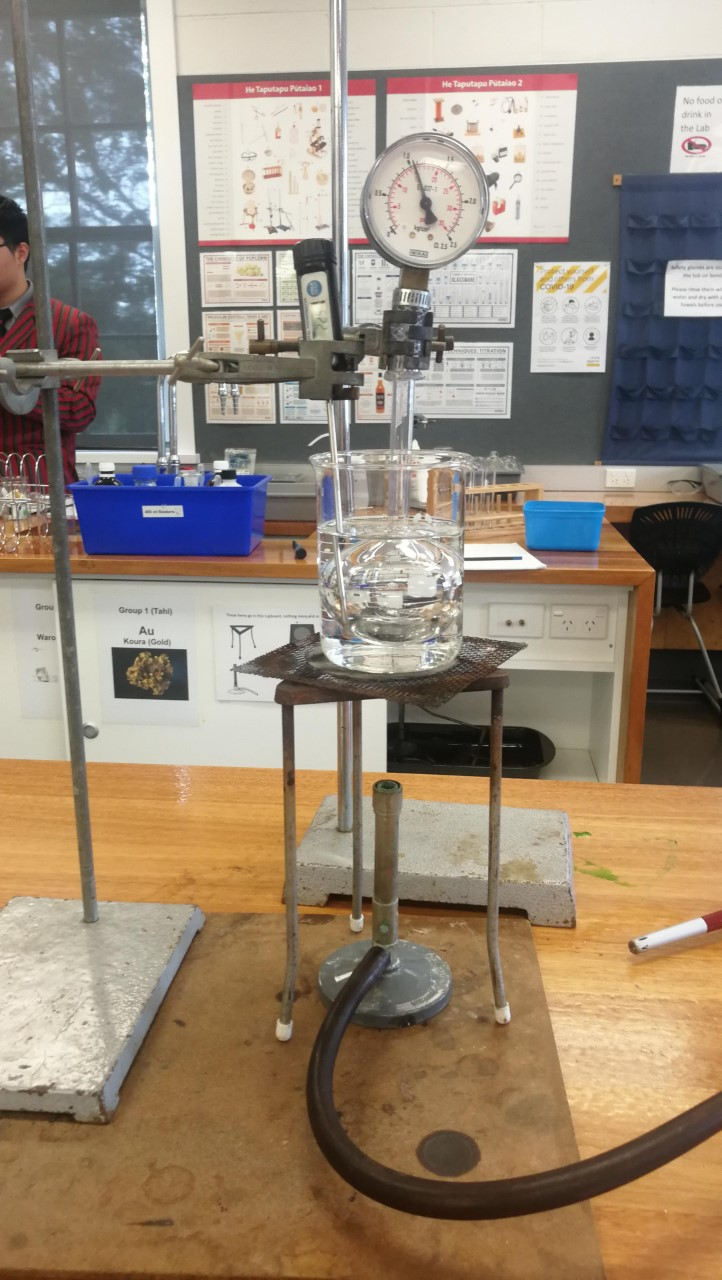
\includegraphics[scale=0.4]{assets/setup.jpg}
 \caption{The experiment setup}
 \label{fig:exp}
\end{figure}




\subsection{Safety}

\section{Data}
\subsection{Raw Data}
\subsection{Processing}

\section{Conclusions}
\subsection{Result}
\subsection{Implications}
\subsection{Reflection}

\end{document}
